\section{Implementazione}

\subsection{Svolgimento della simulazione}
La simulazione svolta consiste in tre esecuzioni distinte di un programma
Protelis all'interno di una rete di dispositivi. Ciascuna di queste simulazioni
è stata eseguita utilizzando una tecnologia differente al fine di realizzare la
comunicazione tra i nodi. Per ragioni di continuità il programma eseguito è
stato sempre il medesimo.

\subsubsection{Topologia della rete}
Per verificare il funzionamento del software è stata simulata una rete di 5
dispositivi, organizzati secondo una topologia ad anello, ovvero disposti a
cerchio e ciascuno può comunicare solo con i dispositivi ad esso
adiacenti. Solo ad uno di questi dispositivi è stata inizializzata una variabile
\texttt{leader} lo distingue dagli altri. Ad ogni dispositivo è assegnato un id
numerico incrementale che parte da 0.

\begin{figure}[H]
  \centering
  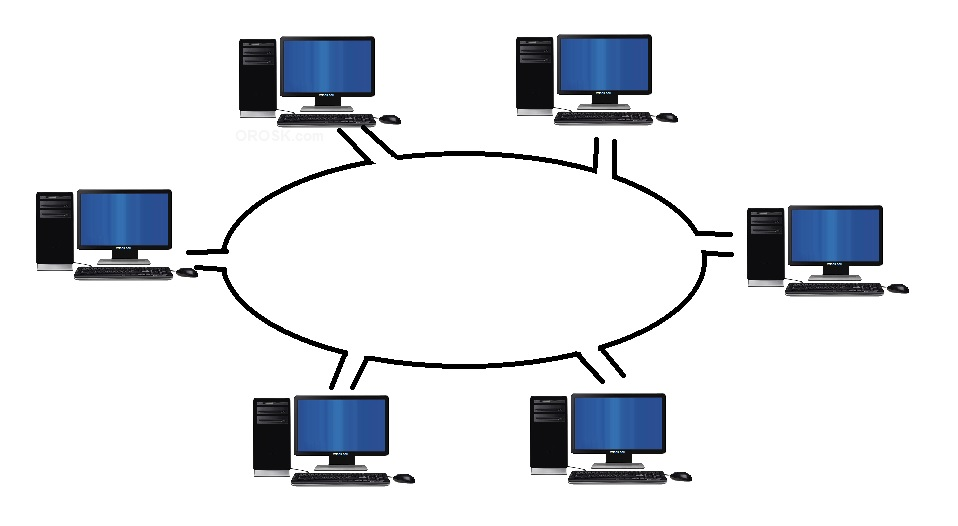
\includegraphics[width=\linewidth]{media/ring-network.jpg}
  \caption{Topologia di rete ad anello}
  \label{fig:1}
\end{figure}

\subsubsection{Descrizione del programma eseguito}
Il programma Protelis eseguito dai dispositivi è il seguente:
\begin{verbatim}
module hello
import protelis:state:time

// Get a variable from the environment
let leader = env.has("leader");

if(leader) {
        self.announce("The leader is at "+self.getDeviceUID().getUid());
        self.announce("The leader's count is: "+countDownWithDecay(4,1));
} else {
        // Otherwise, stay silent
        false;
};

// Check if any neighbor is the leader
if (anyHood(nbr(leader))) {
        // if so, speak!
        self.announce("Hello from the leader to its neighbor at " +
                       self.getDeviceUID().getUid());
} else {
        // Otherwise, stay silent
        false;
};
\end{verbatim}
Nelle prime due righe viene definito il nome del modulo di appartenenza del
programma ed è importato il modulo nel quale è presente la funzione
\texttt{countDownWithDecay()} utilizzata in seguito. Dopodiché la rete viene
divisa in due parti sulla base della variabile booleana \texttt{leader}: la
prima metà --- in questo caso solamente un nodo --- utilizza la funzione
\texttt{announce()} per comunicare il proprio \texttt{DeviceUID} e per svolgere
un conteggio a ritroso da 4 escluso; la seconda metà semplicemente valuta
l'istruzione \texttt{false} per non eseguire alcun codice.
Successivamente la rete viene partizionata nuovamente utilizzando come
discriminante l'espressione \texttt{anyHood(nbr(leader))}, che permette di
selezionare quelli che tra i propri vicini hanno almeno un \textit{leader}.
Questi annunciano la propria vicinanza a un \textit{leader} e il proprio
\texttt{DeviceUID}; i dispositivi che non sono vicini ad un \textit{leader} ---
quindi anche essi stessi --- valuta nuovamente l'istruzione \texttt{false} per
non eseguire nessuna istruzione.


\subsection{Esempio memoria condivisa}

\subsection{Esempio con socket}

\subsection{Esempio con protocollo MQTT}

\subsection{Strumenti di sviluppo}

\subsubsection{Git}
Git è un sistema di controllo versione distribuito, sviluppato da Linus Torvalds
nel 2005 per la gestione del kernel Linux. Grazie alla sue numerose funzionalità
e alla sua semplicità di utilizzo, da allora il suo impiego è stato sempre
crescente fino a quando non ha finalmente conquistato il primato nel
settore\footnote{https://dzone.com/articles/eclipse-community-survey-2014}.

Le sue funzionalità si basano sul concetto di \textit{commit}, ovvero una serie
di aggiunte, modifiche o cancellazioni effettuate sulle righe di uno o più file
di un progetto. I commit sono mantenuti in un determinato ordine e questo
consente di navigare le numerose versioni del software agevolmente. Questo
sistema di gestione delle modifiche permette di gestire in maniera molto
semplice la diramazione e l'eventuale fusione di rami paralleli.

\subsubsection{GitHub}
GitHub è un servizio di hosting per repository. Consente di caricare in un
sistema centrale un repository Git, in modo tale da fornire un punto di
sincronizzazione tra più sviluppatori che lavorano sullo stesso progetto. Allo
stesso tempo è il punto di contatto tra il produttore e il consumatore del
software: infatti consente al creatore di inserire le istruzioni per fruirne o
estenderlo.

GitHub prevede la possibilità di effettuare un \textit{fork} di un
progetto, ovvero di clonarlo sfruttando la capacità di
\textit{branching} di Git. Una volta terminata la risoluzione di
eventuali bug o lo sviluppo di nuove funzionalità viene effettuata una
\textit{pull-request}, una richiesta di fusione di un branch
parallelo. Questa può essere accettata immediatamente o dopo la
richiesta di eventuali modifiche dal mantenitore del repository.
L'integrazione dell'applicazione oggetto di questa tesi al repository
ufficiale di
Protelis\footnote{https://github.com/Protelis/Protelis-Demo/} è stato
effettuato in questo modo.

\subsubsection{Gradle}
Gradle è uno strumento per l'automazione dello sviluppo, che definisce tramite
un DSL basato su Groovy o Kotlin un insieme di compiti, il cui ordine di
esecuzione è definito tramite un grafo aciclico diretto. La capacità di eseguire
dei veri e propri script, contrapposta all'uso di file di definizione di
progetto --- tecnica utilizzata per esempio da Apache Maven ---, estende le
possibilità di questo strumento oltre ogni limite.

Le sue principali funzionalità sono:

\begin{itemize}
\item{gestione di \textit{build} multi-progetto con interdipendenze;}
\item{risoluzione delle dipendenze, evitando di dover includere all'interno del
    repository gli scomodi file \textit{jar}, poiché non adatti per essere
    trattati da Git;}
\item{compilazione del codice sorgente;}
\item{esecuzione di controlli finalizzati a mantenere uno standard della qualità
    del codice;}
\item{esecuzione di test;}
\item{generazione della documentazione.}
\end{itemize}

Questo progetto è composto da 6 sottoprogetti, in ciascuno dei quali è definito
uno script che definisce specifiche le dipendenze.

\subsubsection{IntelliJ IDEA}

IntelliJ IDEA è un ambiente di sviluppo integrato, sviluppato dall'azienda
JetBrains distribuito in due versioni, una con licenza Apache e una commerciale.
È stato progettato con l'obiettivo di essere utilizzato per Java e fornisce un
supporto eccellente per il linguaggio Kotlin e l'impiego di Gradle.

L'impiego di questo strumento ha accelerato lo sviluppo dell'elaborato tramite
funzioni di navigazione all'interno del codice e di refactoring.

\subsubsection{Travis CI}
Travis CI è un servizio di \textit{continuous integration} per testare progetti
ospitati su GitHub. Prevede un piano gratuito per repository open-source, che è
stato impiegato per l'integrazione continua del progetto.

All'interno di un repository deve essere presente un file di configurazione che
definisce il linguaggio utilizzato e le azioni da eseguire. Quando il servizio è
abilitato su un repository, viene notificato da GitHub ogni volta che viene
caricata una nuova versione. Questa viene scaricata e vengono eseguiti i compiti
precedentemente definiti.
